\subsection{GAP-1998 Auger project technical note. Asymmetry of Air Showers at Ground Level \cite{paper_1998}}

La pregunta central sobre lo que se va a trabajar es si es cierto (que sabemos que no) la afirmación que dice Pryke sobre:

“It is frequently assumed that the signals observed when an extensive air shower strikes a ground array depend only on perpendicular distance from the shower axis (core distance)”

$\Rightarrow$ Las primeras cosas que propone es que:

\begin{itemize}
    \item Para eventos muy angulares no sucede que solo depende de la distancia porque al atravesar mas aire se siguen desarrollando aun mas las lluvias (“due to continuing longitudinal development of the cascade”).
    \item Y después habla de lo mas importante que es el hecho de que el efecto del campo geomagnético distorsiona aun en las lluvias mas perpendiculares.
\end{itemize}

Pryke va a mostrar que el efecto geomagnético es predominante en lluvias de $E \geq 10^{19}$eV y $\theta \leq 60^\circ$

$\underline{def:}$ impact parameter: distancia radial respecto al eje en el plano de la lluvia (recordar que esto se proyecta de manera “elíptica” sobre la superficie)

Algo obvio es que: “In fact for non vertical showers (…) as the cascade continues to develop (…) the particles which strike the ground first represent an earlier stage of development than those which arrive later”.

\colorbox{yellow}{
  \parbox{\dimexpr\textwidth-2\fboxsep}{%
  PREGUNTA: actualmente se sigue midiendo solo hasta los $60^\circ$?}}

\colorbox{yellow}{
  \parbox{\dimexpr\textwidth-2\fboxsep}{%
  PREGUNTA: “In fact an air shower cascade disk first grows and then contracts as it passes down through the atmosphere. Ground level is normally beyond the point of maximum development” $\rightarrow$ esto es así??? súper anti-intuitivo
}}

\colorbox{orange}{
  \parbox{\dimexpr\textwidth-2\fboxsep}{%
  RESPUESTA: Actually no, es súper intuitivo, llega un punto donde alcanzan el threshold mínimo para la creación de nuevas partículas y ese es cuando se llega al $X_max$ y ahí solo queda que las partículas de la lluvia choquen y pierdan energía o sean absorbidas por otras de la atmósfera.
}}

Los plots de la Fig 4 parecen razonables (los entiendo), pero los de las Figs 5 y 6 son raros. Lo que entiendo que debería pasar es que a medida que me alejo del eje de la lluvia la proporción de muones tardíos (que se desarrollan mas?) es grande comparado con los tempranos (no termino de entender que quiere decir que podes comparar los tempranos con los tardíos si todos deberían tardar lo mismo en llegar). 

\colorbox{yellow}{
  \parbox{\dimexpr\textwidth-2\fboxsep}{%
  PREGUNTA: como corno llega a decir que lo que espera ver en las distribuciones de partículas (cuando el efecto geomagnético esta apagado) que el efecto de la asimetría temprano-tardía es un primer armónico (sinusoidal?) con supresión en deg=0 y amplificación en $\pm 180^\circ$. (PREGUNTAS NO MUY RELEVANTES)}}

Creo que entendí que es lo que dice $\rightarrow$ vas a ver que el efecto es chico si angularmente estas shallow, ahora, por que es sinusoidal no se?????

Comentario de Juan: este efecto podría no ser tan evidente u observable whatsoever. Esto ya lo dice Pryke, pero no entiendo bien xq. Es por el hecho que el lower limit de la energía necesaria para que los muones decaigan en otras cosas y por ende sigan desarrollándose es grande, entonces llega un punto en el q ya tienen energía por debajo de esto y ya no les da para seguir interactuando entonces siguen de largo. Hipótesis DISCUTIR

Empece a entender un poco el efecto del campo geomagnético (ECG lo voy a llamar por paja de escribir). Te splitea las partículas de carga + y – entonces tenes como dos distribuciones separadas en función de que tanto de modifica el centro.

\colorbox{yellow}{
  \parbox{\dimexpr\textwidth-2\fboxsep}{%
  PREGUNTA: hay efectivamente una diferencia de la carga total de los muones + con – (igual entiendo que no es fácilmente medible la carga de la partícula con los detectores $\rightarrow$ Pryke dice que con los Cherenkov seguro q no y entiendo que con AMIGA tampoco). (PREGUNTAS NO MUY RELEVANTES)}}

Esta conclusión es interesante y piola (asumo que se refiere al valor medio de la distribución porque el ancho debería aumentar): “Hence although the existence of the geomagnetic field may distort the muon charge ratio in the left and right regions the overall muon density is not greatly altered”

\colorbox{yellow}{
  \parbox{\dimexpr\textwidth-2\fboxsep}{%
    PREGUNTA: en el anexo dice devuelta que puede fittear el efecto del ECG como un segundo armónico (dos picos?), why?? (PREGUNTAS NO MUY RELEVANTES)}}


No entendí la ultima frase del paper: “For scintillator detectors the asymmetry would be larger still since they are more reliant on the rapidly attenuating electromagnetic component”.


\subsection{GAP-2002 Towards Parametrization of the Lateral Distribution Function and its Asymmetries in the Surface Detector\cite{paper_2002}}


$\underline{def:}$ Lateral Distribution Function (LDF) is the function that describes empirically the dependence of the signal on the position of the tank with respect to the shower core → is a function of the distance to the core r and of the azimuthal direction (because anisotropies: forward-backward asymmetry and magnetic distortion)

Estoy empezando a preguntarme como es que puedo realizar los mapas de muones en el plano perpendicular a las lluvias, si lo que yo tengo es solamente los detectores subterráneos. La idea es que usando la diferencia temporal entre las detecciones de los diferentes detectores puedo rearmar las lluvias en el plano perpendicular, ponele que te creo eso, pero como hago para extrapolar para atrás en el tiempo como se veían las distribuciones de muones? Es medio raro, no lo entiendo bien. Creo que igual lo que voy a hacer es hacer los mapas sobre la superficie.

Intentando parametrizar esta LDF llegan a una serie de conclusiones:

\begin{itemize}
    \item Para $\theta$ pequeño, la componente electromagnética de la lluvia iniciada por un primario protón, no alcanzo su máximo todavía, frente a lluvias de primarios mas pesados donde la lluvia se ve mas avanzada (‘‘envejecida’’).
    \item Para $\theta$ grande, este efecto es al revés donde las lluvias pesadas son mas avanzadas en su decaimiento que las livianas (protones), pero esto se compensa con la mayor parte muonica de la lluvia que domina para $\theta$ grande
\end{itemize}

Hace un comentario que me pareció relevante para discutir. Dice que las lluvias mas verticales pueden no llegar a ser las mas optimas para la discriminación y que las mejores son las de entre $40^\circ$ y $50^\circ$ donde el "ratio entre tamaño-de-tierra (entiendo que se refiere al detector) / energía es mas favorable". No termino de entender si esto tiene que ver con el hecho de que así   garantizas que las lluvias puedan llegar su $X_{max}$ siempre, pero sin irte a lluvias muy angulares y por ende deformadas ?? Pero no se.

El capitulo 5 es el mas interesante. Habla de varias cosas que creo relevante ir comentando. Primero dice que se va a intentar fittear la asimetría en la detección sobre la superficie como 

\begin{equation}
    S(r,\psi) = \hat{S} (1 + A(r) cos(\psi))
    \label{eq_de_asimetrias}
\end{equation}

Dice que el valor de A desaparece en r=0 lo cual es razonable, porque  sobre el eje no se deforma. Pero después dice algo medio raro, que el valor de A llega a un plateau pero que esto solo lo logran describir empíricamente y no teóricamente (no hay explicación? dice algo como que el problema es que para r grande no hay suficiente estadística). 

Spoiler, yo voy a buscar parametrizar A con no solo la distancia al eje r, sino también con el angulo zenital con el que entra $\theta$.

Una vez q llegan a una parametrizacion dicen esto: "the combination of shower-to-shower variations and satistical fluctuations of the signal in the tank are not negligeble compared to the amplitude of the asymmetry, then a more precise parametrizaction would not really help".

NO ESTOY SEGURO, PERO SUENA Q MANDARON CUALCA

No termino de entender estas frases que dice todo el tiempo de que hay veces que domina la parte muonica.

\subsection{GAP-2022 Extensive air shower asymmetry and
cosmic ray mass composition with the
upgraded Pierre Auger Observatory\cite{tesis_bradfield}}

Frase que me gusta mucho para tener noción de lo raros que son los eventos de alta energía: 

‘‘For comparison, a flux of 1 $particle/m^2/second$ above $10^{14} eV$ drops to approximately 1 $particle/km^2/century$ above $10^{20} eV$.’’

No tiene que ver directamente con la tesis, pero hay varias cosas interesantes que no me había puesto a pensar antes y que son respuestas a preguntas que no me había hecho, por ejemplo por que las UHECR son extra-galácticos: 

“One piece of information the Hillas criterion does allow us to infer is that the lack of measured galactic-plane anisotropy (see Section 1.6) indicates that cosmic rays of the highest energies come from sources which are extra-galactic, such as AGN. This is because protons accelerated to $10^{20}$ eV by a galactic source would have a gyro radius of $\approx$ 100 kpc within the galaxy. This is considerably larger than the radius of the Milky Way at $\approx$ 16 kpc. Therefore, these protons would be expected to travel in nearly straight lines towards Earth, creating a clear hotspot. Since no evidence of such an excess has been observed, the sources for such particles are assumed to be located outside our galaxy”.

Otra cosa mas respecto a las explicaciones de del cutoff de energía a partir de los $10^{19} eV$ que se ve en la Figura puede atribuirse a una de dos cosas (yo entendía que estaba medianamente aceptado que esta asociado al GZK?):

\begin{figure}[!ht]
    \centering
    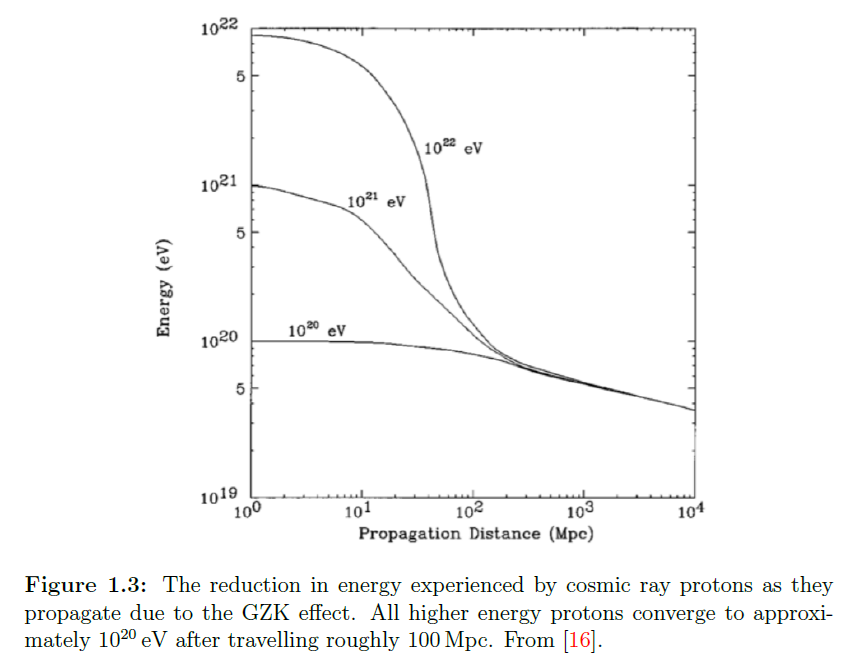
\includegraphics[width=1\linewidth]{Notas Iniciales/GZK.png}
    \label{fig:GZK}
\end{figure}


‘‘As shown in Figure 1.3, these interactions would cause a rapid decrease in energy for any cosmic ray with $E > 10^{20} eV$. This creates a cutoff where, after $\approx 100Mpc$,
any higher energy cosmic ray will converge to $E \approx 10^{20} eV$. An alternative, albeit far less interesting, explanation for the suppression is that sources of cosmic rays cannot accelerate particles to higher energies [15].’’

Otra mas respecto a como es la medición de los primarios en eventos de alta energía donde se usan las EAS:

“(...) the fuctuations in the development of EASs do not allow for the primary composition to be determined on an event by event basis. However by looking at ensembles of showers and their average properties one can estimate the abundance of primaries in 4 mass groups, namely protons (hydrogen), helium, nitrogen and iron. At the highest energies, this is typically done using a shower parameter known as $X_{max}$ essentially a measure of
where in a shower's development the greatest number of particles is observed. The key point is that the $X_{max}$ distributions of lighter primaries, such as proton, have both larger means and standard deviations than heavier primaries like iron. Figure 1.8 shows measurements of the mean and standard deviation of $X_{max}$ distributions as a function of energy from the Pierre Auger Observatory. The lines plotted indicate
predictions based on various hadronic interaction models. When compared with the models, there is a clear change in behaviour around the ankle region, where the
average composition begins to become heavier”.

\begin{figure}[!ht]
    \centering
    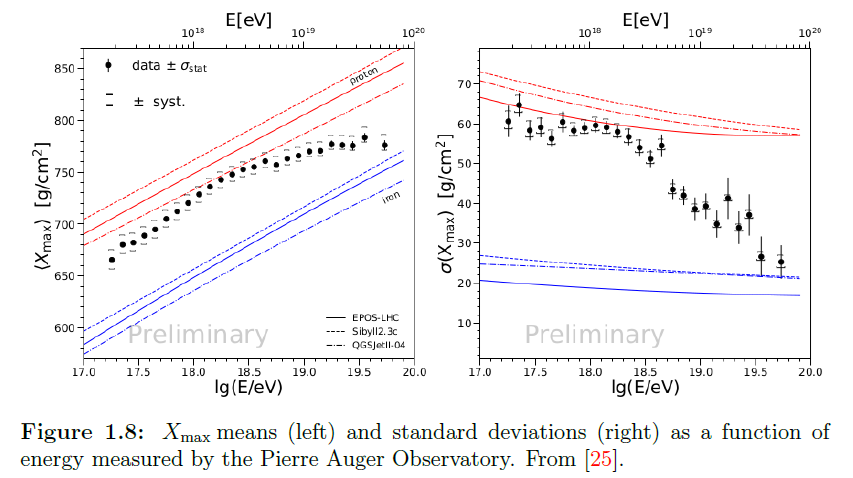
\includegraphics[width=1\linewidth]{Notas Iniciales/X_max_para_light_y_heavy.png}
    \label{fig:X_max}
\end{figure}

Para entender, en el mapa de cielo, cuando se ve que no son isotropicas los UHECR que es ese dipolo del cual se habla? Es la galaxia esta Centauri que menciono el flaco de IB en la charla de la RAFA?

\colorbox{yellow}{
  \parbox{\dimexpr\textwidth-2\fboxsep}{%
    PREGUNTA: Leyendo esto me acorde de una de las preguntas que me hizo Pedro en la RAFA, no sucede en UMD que tenes dos impactos de muones en el tiempo en el que la electrónica responde, mezclándote así las señales de dos eventos diferentes? Es simplemente que esto es improbable por la cantidad de eventos o por la velocidad de respuesta de la electrónica?
}}

\colorbox{orange}{
  \parbox{\dimexpr\textwidth-2\fboxsep}{%
    RESPUESTA: Si pero se logran eliminar con estadística (esta cuantificado cuanto es que pasa y entiendo que es como que lo ‘‘restas’’).
}}

Primer resultado importante que voy a ver si logro replicar respecto a los resultados de la asimetría (entiendo que el parámetro $b$ es el que yo llamo $A$) es: 

‘‘From this plot, we see a clear increase in the magnitude of the asymmetry with zenith angle (in both detectors) for both proton and iron primaries up to the second to last bin, which corresponds to $\approx 50^\circ $. The noticable drop in the asymmetry amplitude in the final bin for each primary/detector type is possibly due to these showers ‘‘running out’’ of electromagnetic particles, which are generally considered to be the primary cause of asymmetry. This may be because of the large amount of atmospheric depth needed to be traversed at large zenith angles. (...) it is evident that the asymmetry is somewhat
greater when measuring showers initiated by proton primaries than iron primaries for zenith angles $\gtrsim 30^\circ ~~(sin^2(\theta) \gtrsim 0.3)$. Again this is probably because of muons,
specically that they constitute a larger portion of the total number of particles in
an iron shower than a proton shower.’’

\begin{figure}[!ht]
    \centering
    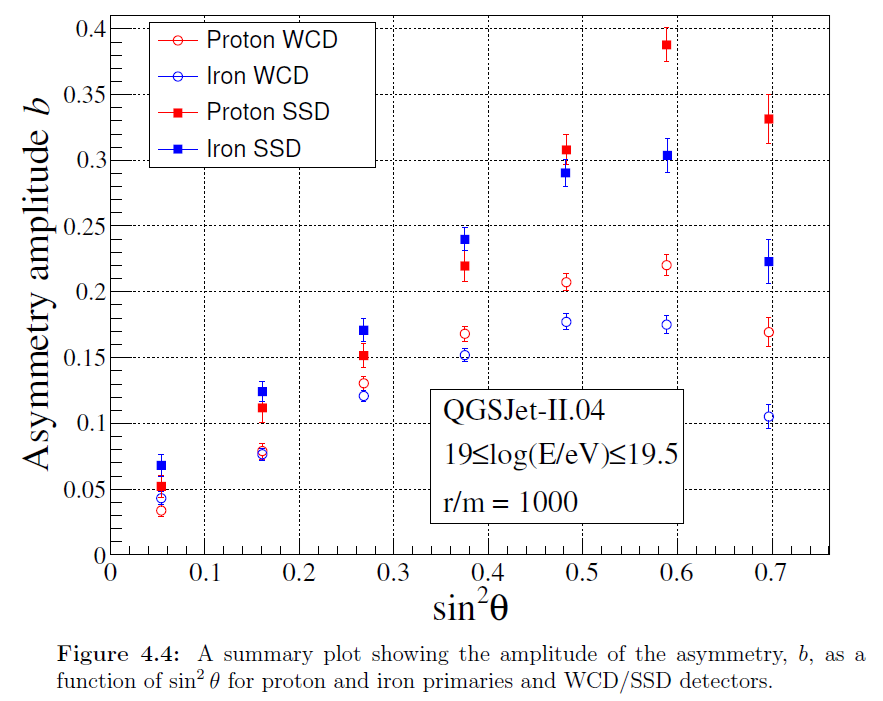
\includegraphics[width=1\linewidth]{Notas Iniciales/asymmetry_amplitude.png}
    \label{fig:asymmetry_amplitude}
\end{figure}

Hay constantemente todo a lo largo de la tesis y de los otros papers frases como estas ‘‘(...) muons, which typically show less asymmetry than electromagnetic particles (...)’’ pero no entiendo por que. Esto lo quiero discutir. Entiendo un poco la razón pero se engancha con las preguntas de antes de que quiere decir que las lluvias se convierten en muónicas y lalala.

Una vez que caracterizo la asimetria comparando lluvias de protones e hierros agarra y se fija cuando son maximas y llega a esto: ‘‘This seems to suggest the maximum difference does not depend significantly on the radius, only on the zenith angle and $log(S_{1000})$.’’€€€¦€€€€€€¦¦¦¦€\\\\\\